\chapter{Поиск предельного цикла}

Познакомимся с исcледуемой системой (уравнение \ref{lab:eq:1},
$\nu$ - параметр системы). Она описывается
уравнением от одной фазовой переменной $x$, уравнение дифференциальное, второго 
порядка и, в силу слогаемого $3\dot{x}^3$, нелинейное. Решение такого уравнения 
аналитическими методами является давольно сложной задачей, поэтому нашим
методом исследования будет построение численых экспириментов, описывающих
данную систему при определенном параметре $\nu$.

\begin{equation}\label{lab:eq:1}
  \ddot{x} + 3 \dot{x}^3 - \nu\dot{x} + x = 0
\end{equation}

Однако, в таком виде уравнение \ref{lab:eq:1} не является удобным для постоения.
Поэтому приведем его к канонической форме от двух
переменных, с помощью замены \ref{lab:eq:2}, получив уравнение от двух фазовых
переменных $y_1$ и $y_2$ (Система уравнений \ref{lab:eq:3}). В дальнейшем,
мы будем пользоваться описанием нашей системы именно в таком виде.

\begin{equation}\label{lab:eq:2}
  \begin{cases}
    &y_1 = x \\
    &y_2 = \dot{x}
  \end{cases}
\end{equation}

\begin{equation}\label{lab:eq:3}
  \begin{cases}
    &\dot{y_1} = y_2 \\
    &\dot{y_2} = -3y_2^3\ + \nu y_2 - y_1
  \end{cases}
\end{equation}

Теперь, зная зависимость значения производных от их координат, можно построить
фазовый портрет с помощью функции \textit{streamplot} из библиотеки 
\textit{matplotlib}
(Программа \ref{lab1:prog:1}, в качестве параметра для начала возьмем $\nu = 1$). % TODO: Ссылка на документацию
Данная функция принимает сетку, на которой проводятся вычисления, и 
значение векторов в каждой точке, после чего, на основе полученных, она рисует
векторное поле, отображая фазовые линии, плотность которых можно регулировать
соответствующим параметром \textit{density}.

В нашем случае, будет естественно взять за значение векторов значения
производных $y_1$ и $y_2$ в данных точках, тем самым мы получим визаулизацию
поведения системы, при определенном параметре. 

\clearpage

\begin{program}
  \caption{Построение фазового портрета}
  \label{lab1:prog:1}
  \begin{verbatim}
# Подключение используемых библиотек
# В дальнейшем является постояным и опускается в листингах
# Полный исходный код программы можно найти в приложении 
import matplotlib.pyplot as plt
import numpy as np

# Параметр системы
nu = 1

# создание сетки 100х100 точек в области [-3;3]x[-3;3]
Y, X = np.mgrid[-3:3:100j, -3:3:100j]

# вычисление фазовых векторов на сетке
Y1 = Y
Y2 = -3 * Y ** 3 + nu * Y - X

# построение фазового портрета
fig0, ax0 = plt.subplots()
plt.streamplot(X, Y, Y1, Y2)

# показать построенные графики (опускается в дальнейшем)
plt.show()    
  \end{verbatim}
\end{program}

\clearpage

\begin{figure}[thp]
  \centering
  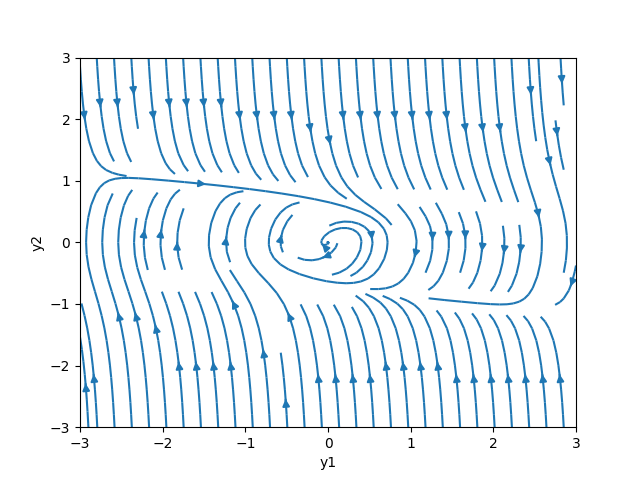
\includegraphics[width=\textwidth]{figures/1_streamplot}
  \caption{Поиск предельного цикла с помощью векторного портрета}
  \label{lab1:streamplot}
\end{figure}

Для начала, найдем хотя бы одно значение параметра, при котором наблюдается 
предельный цикл. Взяв параметр $\nu = 1$, построим фазовый партрет.
Результат работы программы изабражен на рисунке \ref{lab1:streamplot}.
В данном случае, нам повезло с подбором параметра: на рисунке рассматривается
наличие придельного цикла в области $[-1;1]\times[-1;1]$, к которому 
притягиваются все точки системы, т. е. мы наблюдаем наличие аттрактора.

Чтобы убедится, в результатах данного построения, построим две траектории
внутри и во вне наблюдаемого предельного цикла. Для этого воспользуемся
методом Эйлера (Программа \ref{lab1:prog:2}).

\begin{program}
  \caption{Использование метода Эйлера для проверки предельного цикла}
  \label{lab1:prog:2}
  \begin{verbatim}
# функция построение кривой методом Эйлера
def line(y1_0, y2_0):
    y1 = [y1_0]
    y2 = [y2_0]
    h = 0.01 # длина шага
    for i in range(2000): # 200o - количество итераций
        y1.append(y1[-1] + h*(y2[-1]))
        y2.append(y2[-1] + h*(-3*y2[-1] ** 3 + nu*y2[-1] - y1[-1]))
    # отображение кривой на графике
    ax0.plot(y1, y2)

# построение двух кривых, начинающихся внутри и 
# вне предпологаемого предельного цикла
line(0.1, 0.1)
line(2, 2)
  \end{verbatim}
\end{program}

\clearpage

\begin{figure}[thp]
  \centering
  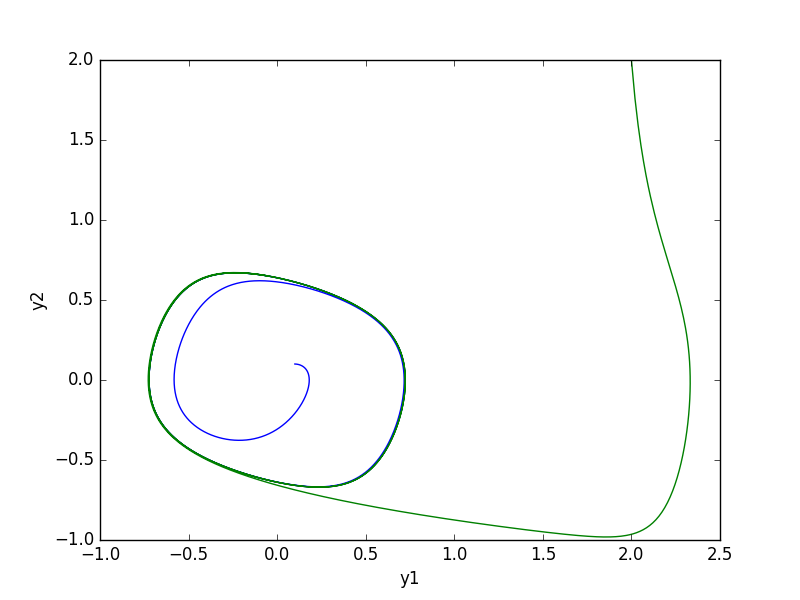
\includegraphics[width=\textwidth]{figures/1_attractor}
  \caption{Обнаружение аттрактора методом Эйлера}
  \label{lab1:attractor}
\end{figure}

На рисунке \ref{lab1:attractor} теперь мы можем видеть, что из точек $(0.1, 0.1)$
и $(2, 2)$ линии сходятся к предельному циклу наблюдаемому ранее.
